\appendix
%%% Оформление заголовков приложений ближе к ГОСТ:
\setlength{\midchapskip}{20pt}
\renewcommand*{\afterchapternum}{\par\nobreak\vskip \midchapskip}
\renewcommand\thechapter{\Asbuk{chapter}} % Чтобы приложения русскими буквами нумеровались


%==============================================================================
%                Свидетельство о регистрации программы для ЭВМ
%==============================================================================
\chapter{Свидетельство о регистрации программы для ЭВМ} \label{appendix:programm_registration}
\begin{figure}[ht]
    \framebox{
\includegraphics[width=0.9\textwidth]{program_registration_no2015660380}}
\end{figure}


%==============================================================================
%                Постановка задачи анализа независимых компонент
%==============================================================================
\chapter{Дополнительный материал} \label{appendix:math}

%==============================================================================
\section{Вывод оригинальной функции активации}  \label{appendix:math:activation_function}

Несмотря на то, что в работе~\cite{EmelyanovYaroslavsky1990} рассматривается стохастическая импульсная модель нейрона, автор так же отмечает, что при рассмотрении \socalled пачки импульсов нейрон можно рассматривать как детерминированный пороговый элемент и усреднённая частота возникновения импульсов будет определяться равенством: $$\text{U}^\text{М} - \text{П}_{0}^\text{Д}(\tau) \cdot \text{П}_{1}^\text{Д}(Q^\Sigma) = 0 ,$$ где $\text{U}^\text{М}$ --- медленный потенциал нейрона, отражающий вклад возбуждающего и тормозного воздействия других нейронов, а так же влияние медленно изменяющихся пороговых величин самого нейрона, $\text{П}_{0}^\text{Д}(\tau)$ --- функция динамического порога, зависящая от прошедшего с момента предыдущего импульса времени $\tau$ и изображённая \onfigure~\ref{fig:ia_thresholds}а, $\text{П}_{1}^\text{Д}(Q^\Sigma)$ --- модулирующая динамический порог функция, зависящая от \socalled самочувствия нейронов сети $Q^\Sigma$ и изображённая \onfigure~\ref{fig:ia_thresholds}б.

\IncludeFigure{ia_thresholds}{Определённые в работе~\cite{EmelyanovYaroslavsky1990}: а) функция динамического порога $\text{П}_{0}^\text{Д}$, зависящая от межспайкового интервала $\tau$; б) модулирующая динамический порог функция $\text{П}_{1}^\text{Д}$, зависящая от параметра самочувствия нейронов $Q^\Sigma$.}

Для удобства введём величину $\bar{\text{U}}^\text{М} = \text{U}^\text{М} / \text{П}_{1}^\text{Д}(Q^\Sigma)$ и примем во внимание, что временной интервал между возникновением импульсов в пачке несоизмеримо мал в сравнении с временем, необходимым для ощутимого изменения медленного потенциала $\text{U}^\text{М}$. Тогда усреднённая частота генерации импульсов $y$ будет определяться выражением: 
$$ y = \dfrac{1}{\tau} = \dfrac{1}{{\text{П}_{0}^\text{Д}}^{-1}(\bar{\text{U}}^\text{М})}.$$

Однако явно использовать обратную функцию ${\text{П}_{0}^\text{Д}}^{-1}(\bar{\text{U}}^\text{М})$ невозможно, т.к. функция $\text{П}_{0}^\text{Д}(\tau)$ не обладает свойством монотонности при $\tau \in \left[ \tau_{1}^{\text{н}}; \tau_{2}^{\text{н}} \right]$. В то же время, основываясь на том, что нас интересуют усреднённые частотные величины, мы можем без потери качественных свойств преобразовать функцию $\text{П}_{0}^\text{Д}(\tau)$ к монотонному виду $f(y)$, изображенному \onfigure~\ref{fig:ia_thresholds_fixed}.

\IncludeFigure{ia_thresholds_fixed}{Функция $f(y)$, являющаяся результатом приведения функции $\text{П}_{0}^\text{Д}(\tau)$, изображённой \onfigure~\ref{fig:ia_thresholds}а, к функционально эквивалентному монотонному виду.}

Далее необходимо формализовать функцию $f(y)$, основываясь на её качественном графическом представлении. Для этого определим её в виде кусочно-гладкой функции, изображённой \onfigure~\ref{fig:ia_activation_function}:
$$
    f(y) = 
    \begin{cases}
        f_{1}(y) = \dfrac{2,6}{1 + e^{\displaystyle -(y - 0,1935) \cdot 120}}   &, y \in \left[0; \frac{1}{3,5}\right]    \\
        f_{2}(y) = k_{12} + \dfrac{0,35}{1 - y}                                 &, y \in \left(\frac{1}{3,5}; 1\right]    \\
    \end{cases}
$$
где коэффициент $k_{12} = 2,6 \cdot \sigma\left(\frac{38,73}{3,5}\right) - 0,49 \approx 2,11$ ($\sigma$ --- логистическая функция) был подобран таким образом, чтобы функция в целом обладала свойством непрерывности, \ie выполнялось условие: $f_{1}(1/3,5) = f_{2}(1/3,5)$. При этом область определения функции $D(f) = \left[0; 1\right]$. В этом случае обратная функция $f^{-1}(y)$ выводится аналитически и имеет вид:
$$
    f^{-1}(u) = 
    \begin{cases}
        f_{0}^{-1}(u) = 0                                                               &, u < u_{01}      \\  
        f_{1}^{-1}(u) = 0,1935 + \dfrac{1}{120} \ln\left( \dfrac{u}{2,6 - u} \right)    &, u_{01} \le u \le u_{12}  \\
        f_{2}^{-1}(u) = 1 - \dfrac{0,35}{x - k_{12}}                                     &, u > u_{12}    \\
    \end{cases}
$$
где $u_{01} = 2,6\cdot\sigma\left(-23,22\right) \approx 0$ и $u_{12} = 2,6 \cdot \sigma\left(\frac{38,73}{3,5}\right) \approx 2,6$.

\IncludeFigure{ia_activation_function}{Вид: а) кусочно-гладкой функции $f(y)$; б) функций $f_{1}(y)$ и $f_{2}(y)$, которые определяют $f(y)$ на интервалах $\left[0; 1/3,5\right]$ и $\left(1/3,5; 1\right]$ соответственно. }

Таким образом, используемая в диссертационной работе \textbf{оригинальная функция активации} определяется как $s(u) = f^{-1}(u)$.

Стоит отметить, что в опубликованных в рамках исследовательской деятельности работах \cite{Prostov2015-OMNN,Prostov2015-MEPhI,Prostov2015-ESU} была использована следующая функция активации:
$$
    \hat{s}(u) = 
    \begin{cases}
        0                                       &, u < 0            \\  
        \dfrac{1}{5,2 + 0,23 \ln(2,6/u - 1)}    &, 0 \le u < 2,6    \\
        \dfrac{1}{1 + 0,35 / (u - 2,46)}        &, u \ge 2,6        \\
    \end{cases}
$$
которая имеет более сложную аналитическую форму, а так же хоть и малые, но разрывы в местах смены функций, что затрудняет её аналитическое исследование. Тем не менее, с точки зрения поиска и оценки качественных свойств нейрона как динамической системы можно говорить об их эквивалентности, что было подтвержденно в том числе численными экспериментами. Для наглядности \onfigure~\ref{fig:figure_963} изображены оба варианта оригинальной функции активации в сравнительной форме.

\IncludeFigure{figure_963}{\todo{Вид : а) функции; б) функции.}}


%==============================================================================
\section{Постановка задачи анализа независимых компонент}  \label{appendix:math:ica_description}

Рассмотрим постановку задачи анализа независимых компонент в стационарном случае. Для этого предположим существование \textit{скрытого} случайного вектора $\vector{s}_{m \times 1}$, который соответствует ненаблюдаемому источнику данных, а также предположим, что для него характерно следующее:
\begin{itemize}
    \item компоненты статистически независимы: $\forall\, i,j\ P(\vector{s}_{i}, \vector{s}_{j}) = P(\vector{s}_{i}) P(\vector{s}_{j})$;
    \item компоненты центрированы: $\forall\, i\ \expectation{\vector{s}_{i}} = 0$;
    \item нормальное распределение имеет не более одной компоненты (в противном случае, согласно центральной предельной теореме, их разделение будет проблематично): $\nexists\, i,j:\ \vector{s}_{i} \sim N\left(0, \sigma_{i}\right), \vector{s}_{j} \sim N\left(0, \sigma_{j}\right)$.
\end{itemize}
В этом случае вектор $\vector{s}$ называется \textbf{вектором независимых компонент}, а его элементы $\vector{s}_{i}$ --- \textbf{независимыми компонентами}. Далее предположим, что \textit{наблюдаемый} случайный вектор $\vector{x}_{n \times 1}$ является результатом смешения компонент вектора $\vector{s}$, \ie: $$\vector{x} = f_{\theta}(\vector{s}) + \vector{\varepsilon},$$ где $f_{\theta}$ --- неизвестная функция смешивания, зависящая от вектора параметров $\theta$, и $\varepsilon \sim N\left(0, \text{diag}\left(\Sigma\right)\right)$ --- нормально распределённый случайный вектор с нулевым математическим ожиданием и дисперсией $\Sigma$, который отражает наличие шума в наблюдаемых данных. Тогда решением задачи \acr{ICA} будет являться нахождение по выборке наблюдаемого случайного вектора $\vector{x}$ обратной функции $F_{\theta}$, такой что: $$\vector{s} = F_{\theta}(\vector{x}).$$ 
В итоге, применение обратной функции $F_{\theta}$ к любой реализации вектора $\vector{x}$ даст значения соответствующих ему независимых компонент $\vector{s}_{i}$. Это означает, что мы получим способ проецирования наблюдаемых векторов в пространство, в котором компоненты векторов обладают свойством статистической независимости, что является следствием определения вектора независимых компонент.

В линейном случае формулировка задачи приобретает вид: $\vector{x} = \matrix{A} \vector{s} + \varepsilon,$ где $\matrix{A}_{n \times m}$ --- матрица смешивания независимых компонент вектора $\vector{s}$. Решением задачи в этом случае будет нахождение обратной матрицы $\matrix{W}$ (а в случае, когда $m > n$, псевдо обратной матрицы), такой что: $\vector{s} = \matrix{W} \vector{x}.$


Для примера, \onfigure~\ref{img:ica_compare_with_pca} изображен результат применения анализа независимых компонент и метода главных компонент к набору данных... Можно отметить, что визуально проекция на пространство независимых компонент выглядит более интересной, чем проекция на пространство главных компонент.

\begin{figure}[ht]
    \makebox[\textwidth][c]{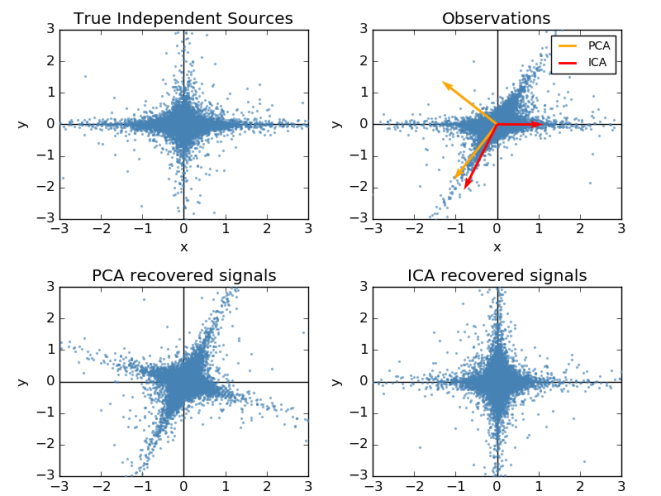
\includegraphics[width=1.0\textwidth]{ica_compare_with_pca}}
    \caption{\todo{Сравнение результата ICA и PCA}.}
    \label{img:ica_compare_with_pca}
\end{figure}
